\section{实验一 \quad 简单流水线与运算器实验}
在进行本次实验前,你需要具备以下实验环境及基础能力:
\begin{enumerate}
    \item 装有\textcolor{red}{Vivado2019.1}的电脑一台;
    \begin{enumerate}
        \item 本实验不对Vivado环境有硬性要求,但涉及Xilinx库中IP的实验,在不同版本环境下无法兼容,且低版本Vivado无法运行高版本生成的项目,为方便实验检查,应当尽量使用实验要求版本。
        \item 若未曾安装Vivado,请参考文档“\textbf{A03\_Vivado安装说明\_v1.00}”。
    \end{enumerate}
    \item 熟悉Vivado的IDE环境,并能够使用其进行仿真、综合;
    \begin{enumerate}
        \item 如果对Vivado不熟悉,参考文档“\textbf{A04\_Vivado使用说明\_v1.00}”。
    \end{enumerate}
    \item 熟悉Nexys4 DDR开发板(Artix-7);
    \\ 请确保在实验进行前阅读过“\textbf{A01\_Nexys4\_DDR用户手册}”。

\end{enumerate}

\subsection{实验目的}

\begin{enumerate}
    \item 理解流水线(Pipeline)设计原理;
    % \item 了解随机存取存储器RAM的原理;
    \item 了解算术逻辑单元ALU的原理;
    % \item 掌握调用Xilinx库IP(Block Memory Generator)实例化RAM的方法;
    \item 熟悉并运用Verilog语言设计ALU;
    \item 熟悉并运用Verilog语言设计流水线全加器;
    \item 学习Verilog不同形式的编程方式,理解assign和always的区别;
\end{enumerate}
\subsection{实验设备}
\begin{enumerate}
    \item 计算机1台(尽可能达到8G及以上内存);
    \item Nexys4 DDR实验开发板;
    \item Xilinx Vivado开发套件(2018.1版本)。

\end{enumerate}

\subsection{实验任务}
本次实验包含两部分,包括ALU设计和简单流水线电路设计。
\subsubsection{ALU设计实验}
图~\ref{fig:alu}给出了一个具有N位输入和N位输出的算数逻辑单元的电路符号。算术逻辑单元接收说明执行哪个功能的控制信号F,执行对应功能后输出N位结果。
\newpage

\begin{figure}[htbp]
    \centering
    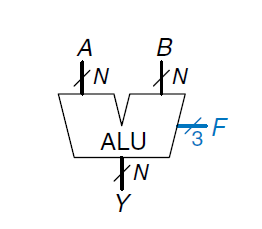
\includegraphics[width = 0.3\textwidth]{image/1_section/alu.png}
    \caption{ALU}
    \label{fig:alu}
\end{figure}

实验要求实现以下算术运算功能,其对应的控制码及功能如下:
\begin{table}[htbp]
    \centering
    \begin{tabular}{cccc}
        \hline
         F$_{2:0}$ & 功能 & F$_{2:0}$ & 功能  \\
         \hline
         000 & A + B(Unsigned) & 100 & $\overline{A}$ \\
         001 & A - B & \textcolor{red}{\textit{\textbf{101}}} & \textcolor{red}{\textit{\textbf{SLT}}}\\
         010 & A AND B & 110 & 未使用\\
         011 & A OR B  & 111 & 未使用\\
         \hline
    \end{tabular}
    \caption{算数运算控制码及功能}
    \label{tab:opcode}
\end{table}

本次实验将ALU输出结果通过板载七段数码管进行显示验证,原理图如图~\ref{fig:alu_experiment}所示:

\begin{figure}[htbp]
    \centering
    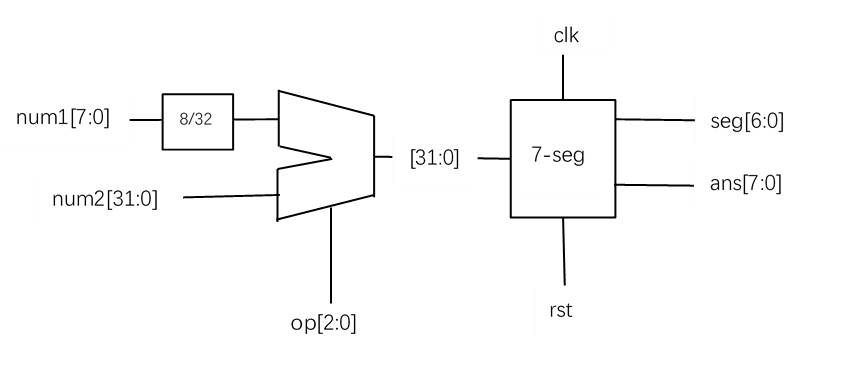
\includegraphics{image/1_section/alu_experiment.png}
    \caption{ALU实验原理图}
    \label{fig:alu_experiment}
\end{figure}

\textbf{实验要求:}
\begin{enumerate}
    \item 根据ALU原理图(图~\ref{fig:alu}),使用Verilog语言定义ALU模块,其中输入输出端口参考实验原理,运算指令码长度为[2:0]。
    \item 自行编写Testbench仿真文件,时钟周期设为10ns,每个时钟周期输入A、B、OP,捕获输出并打印在控制台。\\
        \textcolor{red}{注意:由于疫情原因无硬件设备上板测试,因此不需要做8-32bit扩展。但仍需测试每种运算结果(具体见实验报告表格)。}
    \item 验证表~\ref{tab:opcode}中所有功能。
    \item 实现SLT功能。
    \item 给出RTL源程序(.v文件)
    
    \textcolor{gray}{
    \item 内置一个32位num2(值为32h’01)作为输入到运算器端口A;
    \item 将sw0-sw7输入到num1,经过无符号扩展 至32位后,输入到运算器的端口B;
    \item 运算器支持“加、减、与、或、非”5种运算,需要3位(8个操作)。将sw15-sw14输入到op作为运算器的控制信号;
    \item 将计算32位结果s显示到七段数码管(16进制)。\\     
        \textbf{灰色部分由于疫情原因暂不实现}
    }

\end{enumerate}

\subsubsection{流水线实验}

本次实验为仿真实验,设计完成后仅需进行\textbf{行为仿真}。

\textbf{实验要求:}

% 本次实验使用Vivado的Block Memory Generator模拟数据在存储器中的存取过程。实验使用单端口ROM。初始化ROM存储器中的内容,通过开关选择相应的地址,将对应的存储器中内容读出来,并通过七段数码管显示。实验原理如图~\ref{fig:memory_experiment}所示:

% \begin{figure}[htbp]
%     \centering
%     \includegraphics[width = \textwidth]{image/1_section/memory_experiment.png}
%     \caption{Caption}
%     \label{fig:memory_experiment}
% \end{figure}

% \textbf{实验要求:}
\begin{enumerate}
    \item 实现4级流水线32bit全加器,每一级进行8bit加法运算,需\textcolor{red}{带有流水线暂停和刷新};
    \item 模拟流水线暂停,仿真时控制10周期后暂停流水线2周期(第2级),流水线恢复流动;
    \item 模拟流水线刷新,仿真时控制15周期时流水线刷新(第3级)。

\end{enumerate}

\subsection{实验环境}
以下表格中红色部分需自行实现,黑色部分与实验发布包中提供。

\subsubsection{ALU实验}

\begin{table}[htbp]
    \centering
    \begin{tabu}{|l|l|}
        \hline
        \textcolor{red}{|--top.v}& 设计顶层文件,参照图~\ref{fig:alu_experiment}将各模块连接。 \\
        \textcolor{red}{|----alu.v}& ALU模块,本次实验重点。 \\
        \rowfont{\color{gray}}
        |----display.v& 七段数码管显示模块文件,已提供。 \\
        \rowfont{\color{gray}}
        |------seg7.v& 七段数码管显示模块组成文件,已提供。 \\
        \rowfont{\color{gray}}
        |--constr.xdc&综合实现时,约束文件,已提供。  \\
        
        \rowfont{\color{red}}
        |--sim.v
        & 仿真文件,控制时钟、信号。 \\
        \hline
    \end{tabu}
    \caption{ALU实验文件树}
    \label{tab:alu_file_tree}
\end{table}

\subsubsection{流水线实验}



\begin{table}[htbp]
    \centering
    \begin{tabular}{|l|l|}
        \hline
        \textcolor{red}{|--sim.v} & 仿真文件,控制时钟、信号。 \\
        \textcolor{red}{|----stallable\_pipeline\_adder.v} & 有阻塞4级流水线8bit全加器实现文件 \\
        % |----ram.coe & RAM初始化文件,已提供 \\
        % |----display.v & 七段数码管显示模块文件,已提供。 \\
        % |------seg7.v & 七段数码管显示模块组成文件,已提供。 \\
        % |--constr.xdc & 综合实现时,约束文件,已提供。 \\
        \hline
    \end{tabular}
    \caption{流水线实验文件树}
    \label{tab:pipeline_file_tree}
\end{table}